\documentclass{VUMIFPSbakalaurinis}
\usepackage{algorithmicx}
\usepackage{algorithm}
\usepackage{algpseudocode}
\usepackage{amsfonts}
\usepackage{amsmath}
\usepackage{bm}
\usepackage{caption}
\usepackage{color}
\usepackage{float}
\usepackage{graphicx}
\usepackage{listings}
\usepackage{subfig}
\usepackage{wrapfig}
\usepackage{makecell}
\usepackage{forest}
\usepackage{pgfplots}

\usepackage{enumitem}
\setlist[1]{itemsep=-2pt}

\renewcommand\theadfont{\bfseries}
\newcommand\tab[1][1cm]{\hspace*{#1}}


\definecolor{myyellow}{RGB}{154, 125, 10}
\definecolor{myred}{RGB}{199, 0, 57}
\definecolor{myblue}{RGB}{52, 152, 219}
\definecolor{mygreen}{RGB}{30, 132, 73}


% Titulinio aprašas
\university{Vilniaus universitetas}
\faculty{Matematikos ir informatikos fakultetas}
\department{Programų sistemų katedra}
\papertype{Bakalauro darbas}
\title{Gestų kalbos vienetų atpažinimas iš video srauto}
\titleineng{Recognition of Sign language units from a video stream}
\author{Pranciškus Ambrazas}
\supervisor{j. asist. Linas Petkevičius}
\reviewer{dr. Vytautas Valaitis}
\date{Vilnius – \the\year}

% Nustatymai
% \setmainfont{Palemonas}   % Pakeisti teksto šriftą į Palemonas (turi būti įdiegtas sistemoje)
\bibliography{bibliografija}

\begin{document}
\maketitle

%% Padėkų skyrius
% \sectionnonumnocontent{}
% \vspace{7cm}
% \begin{center}
%     Padėkos asmenims ir/ar organizacijoms
% \end{center}

\sectionnonumnocontent{Santrauka}
Glaustai aprašomas darbo turinys: pristatoma nagrinėta problema ir padarytos
išvados. Santraukos apimtis ne didesnė nei 0,5 puslapio. Santraukų gale
nurodomi darbo raktiniai žodžiai. 
% Nurodomi iki 5 svarbiausių temos raktinių žodžių (terminų).
% Vienas terminas gali susidėti iš kelių žodžių.
\raktiniaizodziai{neuroniniai tinklai, konvoliuciniai neuroniniai tinklai, rekurentiniai neuroniniai tinklai, apsimokančios sistemos, gestų kalba, lietuvių gestų kalba}   

\sectionnonumnocontent{Summary}
Santrauka anglų kalba. Santraukos apimtis ne didesnė nei 0,5 puslapio.
\keywords{neural networks, convolutional neural networks, recurrent neural networks, machine learning, sign language, lithuanian sign language}

\tableofcontents

\sectionnonum{Įvadas}
Pasaulyje yra virš 7 milijardų žmonių, kurie kasdien tarpusavyje komunikuoja. Netgi 5\% visos žmonijos populiacijos sudaro žmonės, turintys klausos problemų. Vien 34 milijonai iš jų yra vaikai, iš kurių net 60\% praradusių klausą vaikystėje galėjo būti girdintys dabar, jei būtų imtąsi atitinkamų prevencinių priemonių. Paskaičiuota, kad iki 2050 metų žmonių, turinčių šias problemas, skaičius išaugs netgi iki 900 milijonų, o vien šiuo metu 1,1 milijardo jaunų žmonių nuo 11 iki 35 metų amžiaus yra ant klausos praradimo ribos dėl per didelio triukšmo \cite{WhoInt}.

\subsectionnonum{Gestų kalba}
Gestų kalba – tai geriausias būdas klausos negalią turintiems žmonėms bendrauti tarpusavyje. Ja pasaulyje bendrauja didžioji dalis klausos sutrikimus turinčiųjų, o amerikiečių gestų kalba (\textit{angl. American Sign Language (ASL)}) yra trečia pagal populiarumą Amerikoje po anglų ir ispanų kalbų, kuria kalba virš 500 tūkstančių žmonių. Kiekviena šalis turi savo valstybinę kalbą - lietuvių, anglų, ispanų, rusų. Lygiai taip pat kiekviena šalis turi ir savo gestų kalbą. Tai yra tiek jau minėta amerikiečių gestų kalba (ASL), lietuvių, argentiniečių ir kitos gestų kalbos. Netgi tam tikri šalių regionai turi specifinius tos pačios kalbos dialektus, kaip, tarkime, vien Lietuvoje yra aukštaičių, žemaičių, suvalkiečių ar dzūkų tarmės. 

Kiekviena gestų kalba turi savo atskirą gramatiką ir sintaksę. Skirtingos gestų kalbos skiriasi tiek abėcėlėmis, tiek pačiais gestais, dėl to skiriasi netgi ta pati gramatika. Taip yra dėl to, kad nėra bendrinės gestų kalbos - vien Amerikoje yra virš 35 skirtingų gestų kalbų. 

Vienas gestas turi turėti kelias prasmes. Kaip ir lietuvių kalboje žodis „kasa“ turi tris skirtingas reikšmes, taip ir gestų kalboje vienas gestas gali turėti keletą reikšmių. Tačiau iš kitos pusės gestas, parodytas truputėlį kitaip gali turėti visiškai priešingą reikšmę. Tarkime, ASL gestai „geras“ ir „blogas“ skiriasi tik puse į kurią atsuktas deltas, tačiau daugiau neturi jokių skirtumų.

\subsectionnonum{Gestų kalbos specifika}
Kiekviena gestų kalba susideda iš \textbf{trijų} pagrindinių dalių:
\begin{enumerate}
	\item\textbf{Statinė gestų kalba} - dar kitaip vadinama \textit{pirštų kalba} (\textit{angl. fingerspelling}). Tai įvairūs gestai rodomi vienos (ASL, LGK) ar net ir dviejų (britų ar vokiečių gestų kalba) rankų pagalba. Tai nejudantys gestai, rodantys vieną raidę (\textit{žr. \ref{img:asl} pav.}) ar net vieną žodį, kaip, pavyzdžiui, ASL „\textit{I love you}“\footnote{liet. Aš tave myliu} gestas. Yra galimybė žodžius išreikšti ir abėcėliškai. Lygiai taip pat žmonės kasdieninėje kalboje turi galimybę pasakyti paraidžiui. Tačiau yra įprasta jungti raides į žodžius. O žodžius galiausiai į sakinius. Vienas iš variantų, kuomet naudojama gestų kalba paraidžiui tai vardų pasakyme. Tačiau gestakalbiai prisistatydami parodo gestą, kuris priklauso tik jiems. Tai tarsi parašas tam, kad nebereikėtų kreipiantis ar apibūdinant žmogų jo vardo sakyti paraidžiui.
	
\begin{figure}[H]
    \centering
    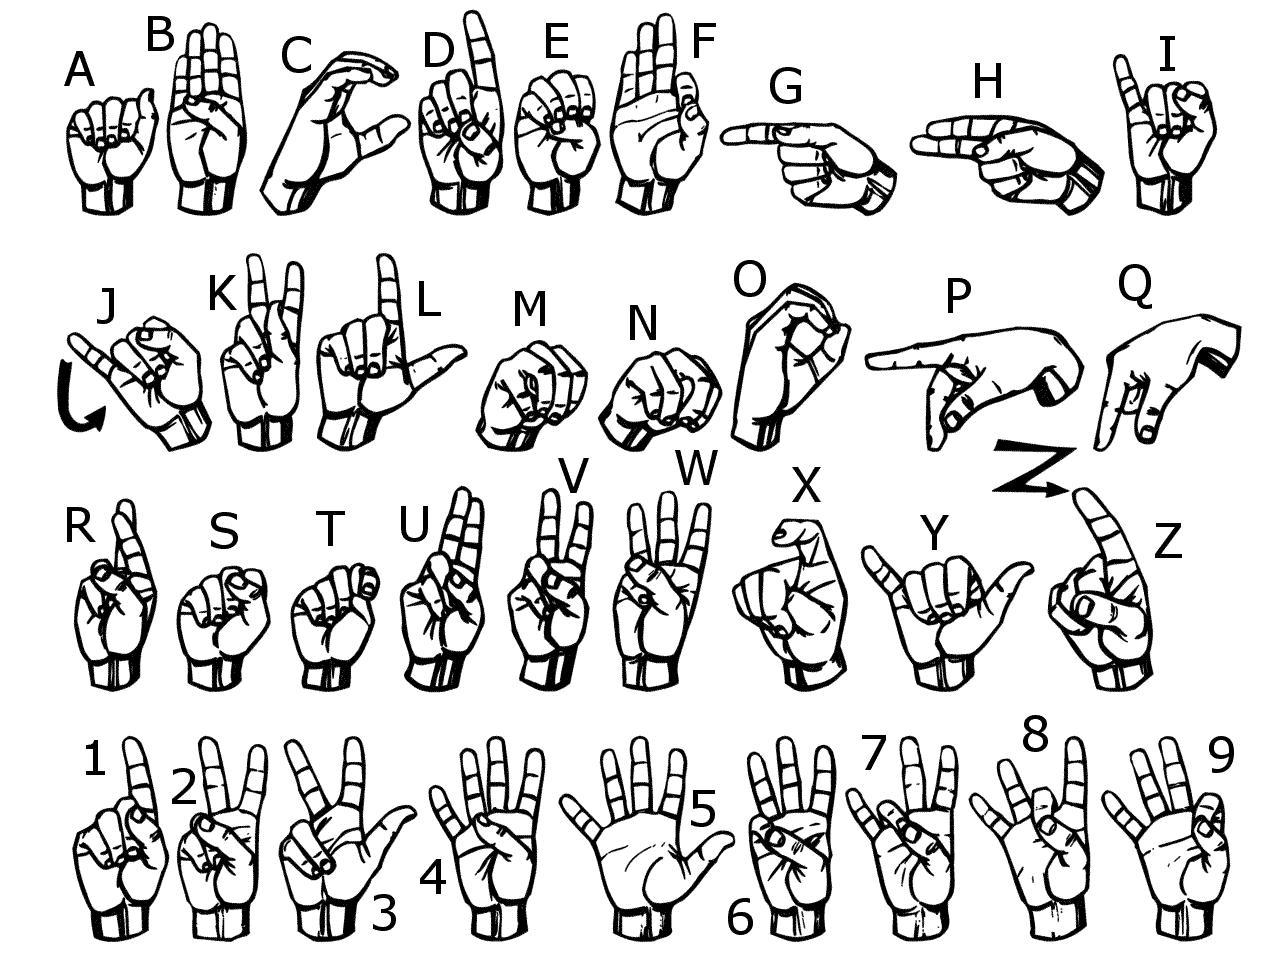
\includegraphics[scale=0.2]{img/ASL}
    \caption{Amerikiečių gestų kalbos abėcėlė}
    \label{img:asl}
\end{figure}

	\item\textbf{Dinaminė gestų kalba} - tai žodžių lygio gestų kalba. Nesunku pastebėti, kad \ref{img:asl} paveikslėlyje yra „J“ ar „Z“ raidės, kurios priskiriama dinaminių judesių klasei. Kaip ir yra žodžių, kurie priskiriami statinei gestų kalbai dėl savo kilmės, taip ir yra raidžių, kurios priskiriamos dinaminei gestų kalbai. Dinaminiais judesiais yra išreiškiami įvairūs gestų kalbos žodžiai tokie, kaip, pavyzdžiui, ASL yra „labas“, „gerai“ ar „blogai“.
	
	\item\textbf{Kitos ypatybės} - emocijos veide, liežuvis, burna ir kūno laikysena. Tai taip pat labai svarbios gestų kalbos ypatybės. Pavyzdžiui, klausiant gestų kalba klausimo, jei bus pakelti antakiai, tai reikš, kad laukiamas ataskymas „taip“ arba „ne“. Tačiau, jei antakiai bus suraukti, tai reikš, kad klausiama su paaiškinimu „kas“, „kur“, „kaip“, „ką“.
\end{enumerate}


\subsectionnonum{Darbo tikslas}
Išanalizuoti gestų kalbos vienetų atpažinimo galimybes ir video srauto.

\subsectionnonum{Darbo uždaviniai}
\begin{itemize}
	\item Gestų kalbos video srautų paieška ir mokomosios medžiagos neuroniniams tinklams surinkimas
	\item Susipažinimas su rekurentiniais neuroniniais tinklais
	\item Gestų kalbos vienetų atpažinimas iš video srauto pasinaudojant rekurentiniais neuroniniais tinklais.
\end{itemize}

\subsectionnonum{Darbo eiga}
\begin{itemize}
	\item Panašių ir jau įgyvendintų projektų paieška
	\item Esamos sistemos patobulinimai
	\item Rezultatų palyginimai
\end{itemize}

\subsectionnonum{Panaudotos priemonės}
\begin{itemize}
	\item Python – programavimo kalba
	\item TensorFlow – skirta darbui su apsimokančiomis sistemomis\footnote{angl. Machine learning}
\end{itemize}



Įvade nurodomas darbo tikslas ir uždaviniai, kuriais bus įgyvendinamas tikslas,
aprašomas temos aktualumas, apibrėžiamas tiriamasis objektas akcentuojant
neapibrėžtumą, kuris bus išspręstas darbe, aptariamos teorinės darbo prielaidos
bei metodika, apibūdinami su tema susiję literatūros ar kitokie šaltiniai,
temos analizės tvarka, darbo atlikimo aplinkybės, pateikiama žinių apie
naudojamus instrumentus (programas ir kt., jei darbe yra eksperimentinė dalis).
Darbo įvadas neturi būti dėstymo santrauka. Įvado apimtis 2–4 puslapiai.


\section{Apsimokančios sistemos}
\textbf{Apsimokančios sistemos} (\textit{angl. machine learning})

\subsection{Prižiūrimas mokymas}
\textbf{Prižiūrimas mokymas} (\textit{angl. supervised learning}) - tai apsimokančių sistemų apmokymo būdas, kuomet duomenys mokymui yra paruošiami taip, kad kiekvienas duomuo turėtų ir atitinkamą rezultatą. Kitaip tariant, jei yra duomuo \textit{a}, tai yra ir jį atitinkantis rezultatas, arba dar vadinama etiketė \textit{b}. Tai būdas, kuris veikia medžio principu.

\begin{table}[H]\footnotesize
  \centering
  \caption{Pavyzdinis prižiūrimo mokymo apmokymui paruoštų duomenų rinkinys}
  {\begin{tabular}{| c | c | c | c | c | c || c |} \hline
    \thead{Nr.} & \thead{Pirštas nr. 1} & \thead{Pirštas nr. 2} & \thead{Pirštas nr. 3} & \thead{Pirštas nr. 4} & \thead{Pirštas nr. 5} & \thead{Raidė} \\
    \hline
    1. & Atlenktas & Užlenktas & Užlenktas & Užlenktas & Užlenktas & \thead{A} \\
    2. & Užlenktas & Atlenktas & Atlenktas & Atlenktas & Atlenktas & \thead{B} \\
    3. & Atlenktas & Sulenktas & Sulenktas & Sulenktas & Sulenktas & \thead{C} \\
    4. & Užlenktas & Atlenktas & Užlenktas & Užlenktas & Užlenktas & \thead{D} \\
    5. & Užlenktas & Užlenktas & Užlenktas & Užlenktas & Užlenktas & \thead{E} \\
    6. & Atlenktas & Užlenktas & Atlenktas & Atlenktas & Atlenktas & \thead{F} \\
    \hline
  \end{tabular}}
  \label{tab:priziurimasPavyzdys}
\end{table}

\ref{tab:priziurimasPavyzdys} lentelėje pateikiamas pavyzdys su amerikiečių gestų kalbos abėcėle. Lentelėje pateikiamos piršų padėtys, o pirštai numeruojami pagal \ref{appendix:pirstai} priede pateikiamą pirštų numeraciją. Kiekvieno piršto padėtis šiame pavyzdyje gali būti: \textit{atlenktas, sulenktas, užlenktas}. Ir kiekvienai padėčiai esant pateikiamas rezultatas, arba kitaip - etiketė, kokią raidę abėcėlėje atitinka pavaizduotos pirštų padėtys.


\begin{table}[H]\footnotesize
  \centering
  \caption{Pavyzdinė praktinė užduotis}
  {\begin{tabular}{| c | c | c | c | c | c || c |} \hline
    \thead{Nr.} & \thead{Pirštas nr. 1} & \thead{Pirštas nr. 2} & \thead{Pirštas nr. 3} & \thead{Pirštas nr. 4} & \thead{Pirštas nr. 5} & \thead{Raidė} \\
    \hline
    1. & Atlenktas & Sulenktas & Sulenktas & Sulenktas & Sulenktas & \thead{?} \\
    \hline
  \end{tabular}}
  \label{tab:priziurimasUzdavinys}
\end{table}

\ref{tab:priziurimasUzdavinys} lentelėje pateikiamas uždavinys, kuriame nurodoma ta pati informacija, kuri buvo pateikta \ref{tab:priziurimasPavyzdys} lentelėje. Tačiau rezultatas nėra pateiktas, o jis randamas medžio principu.


\begin{figure}[H]
    \centering
    
\begin{forest}
  for tree={
    fit=band,% spaces the tree out a little to avoid collisions
  }
  [\textit{Pirštas nr. 1}
    [Atlenktas
      [\textit{Pirštas nr. 2}
      	[Sulenktas [\textbf{C}]]
	[Užlenktas
	  [\textit{Pirštas nr. 3}
	    [Atlenktas [\textbf{F}]]
	    [Užlenktas [\textbf{A}]]
	  ]
	]
      ]
    ]
    [Užlenktas
      [\textit{Pirštas nr. 2} 
      	[Atlenktas
	  [\textit{Pirštas nr. 3}
	    [Užlenktas [\textbf{D}]]
	    [Atlenktas [\textbf{B}]]
	  ]
	]
      	[Užlenktas [\textbf{E}]]
      ]
    ]  
  ]
\end{forest}
    \caption{Galimybių medis}
    \label{img:medis}
\end{figure}


Vien iš šio medžio galimybių medžio galima matyti, kad pilnai užtenka sprendimui nusakyti 3 pirštų, kadangi rezultatų nėra daug. Jei būtų imama visa abėcėlės aibė, tuomet rezultato nustatymui būtų naudojama galimai visų pirštų padėtys. Tačiau net ir šį medį optimizavus galima būtų, tarkime, C raidė atsakymą gauti tik iš vieno piršto padėties, kadangi tik ši vienintelė raidė turi sulenkto piršto padėtį. Galiausiai iš šio medžio galima pastebėti, kad \ref{tab:priziurimasPavyzdys} lentelėje pateikto pavyzdžio atsakymas yra raidė \textbf{C}.

\subsection{Neprižiūrimas mokymas}
\textbf{Neprižiūrimas mokymas} (\textit{angl. unsupervised learning}) - mokymas, kuomet duomenims nėra priskiriamos teisingos etiketės ar teisingi rezultatai. Pavyzdžiui, tai galėtų atitikti naujos kalbos mokymąsi be mokytojo ir bet kokio žodyno. Kuomet pastoviai matomas vis tas pats tekstas, žodžiai tampa atpažįstami, tačiau išversti jų neišeina. Tačiau tai nesukelia jokių nepatogumų, jei į tekstą reikia įrašyti tinkamą žodį, kuomet dėl daugybės duomenų yra aišku koks žodis su kokia galūne turėtų būti įrašytas.

\begin{table}[H]\footnotesize
  \centering
  \caption{Pavyzdinis neprižiūrimo mokymo apmokymui paruoštų duomenų rinkinys}
  {\begin{tabular}{| c | c | c | c | c | c |} \hline
    \thead{Nr.} & \thead{Pirštas nr. 1} & \thead{Pirštas nr. 2} & \thead{Pirštas nr. 3} & \thead{Pirštas nr. 4} & \thead{Pirštas nr. 5}  \\
    \hline
    1. & Atlenktas & Užlenktas & Užlenktas & Užlenktas & Užlenktas  \\
    2. & Užlenktas & Atlenktas & Atlenktas & Atlenktas & Atlenktas  \\
    3. & Atlenktas & Sulenktas & Sulenktas & Sulenktas & Sulenktas \\
    4. & Užlenktas & Atlenktas & Užlenktas & Užlenktas & Užlenktas \\
    5. & Užlenktas & Užlenktas & Užlenktas & Užlenktas & Užlenktas \\
    6. & Atlenktas & Užlenktas & Atlenktas & Atlenktas & Atlenktas \\
    \hline
  \end{tabular}}
  \label{tab:nepriziurimasPavyzdys}
\end{table}

\ref{tab:nepriziurimasPavyzdys} lentelėje pateikiamas pavyzdinis neprižiūrimam mokymui apmokyti paruoštų duomenų rinkinys. Duomenys tokie patys, kaip ir \ref{tab:priziurimasPavyzdys} lentelėje, tačiau nėra teisingo atsakymo sulpelio \textbf{„Raidė“}. Apmokius tokią sistemą būtent tokiais duomenimis vienas iš tikėtinų scenarijų, kur galima būtų panaudoti tokią sistemą, tai nuspėti, kokios raidės yra labiausiai tikėtinos ar tiesiog numatyti, kokia labiausiai tikėtina raidžių seka bus rodoma.


\subsection{Praktinis mokymas}
\textbf{Praktinis mokymas} (\textit{angl. reinforcement learning}) - labiausiai dirbtinį intelektą atitinkančių apsimokančių sistemų apmokymo modelis. Šis mokymas pagrįstas praktiniais bandymais. Kiekvienas teisingai gautas rezultatas yra būdas, kuriuo reikėtų sekti, ir kiekvienas blogai gautas rezultatas, yra būdas, kurio vertėtų atsisakyti. Dažniausiai šis apmokymo būdas naudojamas sistemą apmokant žaisti žaidimus. Vienas iš labiausiai žinomų būtent šiuo apmokymo būdu apmokytų modelių yra \textit{AlphaZero}, kuris sugeba laimėti prieš pasaulio šachmatų čempionus. Tai puikus pavyzdys to, kaip kompiuteris iš laimėjimų, už kuriuos gauna taškus, ir pralaimėjimų, už kuriuos jam taškai atimami, sugeba rasti laimėjimo strategijas kiekviename žingsnyje ir taip, nuolatos tobulėdamas, laimėti dvikovas ar apskritai spręsti uždavinius, kuriuose reikalingas pastabumas ir strategijų kūrimas.


\section{Neuroniniai tinklai}
Žmogaus smegenys yra labai sudėtingas, nelijinis ir paralelinis kompiuteris \cite{Hay09}. Kiekvieno kūnas yra sudarytos iš milijardų nervinių ląstelių vadinamų neuronais. Jie sukuria ir/arba perduoda elektrocheminius impulsus. Neuronai tarpusavyje yra sujungti dendritais, ant kurių yra sinapsės. 

Kiekvienas sužadintas neuronas dėl pasikeitusios temperatūros, spaudimo, skausmo ar kitų veiksnių, perduoda informaciją į smegenis dėl sprendimo, ką daryti, priėmimo. Tai, kaip ir buvo paminėta, yra siųsti signalą iš vieno neurono į kitą, kol galiausiai signalas pasiekia smegenis. Svarbu ir tai, kad kiekvienas neuronas yra nepriklausomas nuo kito. Tai tik grandis, kuri yra atsakinga už signalo priėmimą ir perdavimą. Smegenims gavus signalą, jį apdorojus ir priėmus sprendimą, signalas tuo pačiu keliu siunčiamas atgal, kol pirmąjį sužadinimą gavęs neuronas sulaukia atsakymo. 

\subsection{Perceptronas}

Parceptronas (\textit{angl. perceptron}) – kompiuterinis modelis, skirtas atkartoti žmogaus smegenų darbą. Toliau pateikiamas perceptrono pavyzdys.

\begin{figure}[H]
	\centering
	\tikzset{%
		every neuron/.style={
			circle,
			draw,
			minimum size=1cm
		},
	}
	
	\begin{tikzpicture}[x=1.5cm, y=1.5cm, >=stealth]
	\centering
	
	\foreach \m/\l [count=\y] in {1,2,3,4}
	\node [every neuron/.try, neuron \m/.try] (input-\m) at (0,2.5-\y) {};
	
	\foreach \m [count=\y] in {1,2,3,4}
	\node [every neuron/.try, neuron \m/.try ] (weight-\m) at (2,2.5-\y) {};
	
	\foreach \m [count=\y] in {1}
	\node [every neuron/.try, neuron \m/.try ] (sum-\m) at (4,1.6-\y*1.6) {};
	
	\foreach \m [count=\y] in {1}
	\node [every neuron/.try, neuron \m/.try ] (funk-\m) at (6,1.6-\y*1.6) {};
	
	\foreach \m [count=\y] in {1}
	\node [every neuron/.try, neuron \m/.try ] (output-\m) at (8,1.6-\y*1.6) {};
	
	\foreach \i in {1,...,4}
	\draw [->] (input-\i) -- (weight-\i);
	
	\foreach \i in {1,...,4}
	\draw [->] (weight-\i) -- (sum-1);
	
	\draw [->] (sum-1) -- (funk-1);
	
	\draw [->] (funk-1) -- (output-1);
	
	\foreach \l [count=\x from 0] in {Įeigos\\, Svoriai\\, Suma\\, Aktyvacijos\\funkcija, Išeiga\\}
	\node [align=center, above] at (\x*2,2) {\l};
	
	
	\draw (0,1.49) node {$i_1$};
	\draw (0,0.49) node {$i_2$};
	\draw (0,0.045) node {$\vdots$};
	\draw (0,-0.51) node {$i_n$};
	\draw (0,-1.51) node {$1$};
	
	\draw (2,1.49) node {$w_1$};
	\draw (2,0.49) node {$w_2$};
	\draw (2,0.045) node {$\vdots$};
	\draw (2,-0.51) node {$w_n$};
	\draw (2,-1.51) node {$b$};
	
	\draw (4,0) node {$\sum$};
	
	\draw (6,0) node {$f(x)$};
	
	\draw (8,0) node {$o$};
	\end{tikzpicture}
	\caption{Perceptrono pavyzdys} \label{fig:perceptron}
\end{figure}

\ref{fig:perceptron} paveikslėlyje pavaizduotame pavyzdyje esančią išeigą galima aprašyti formule:
\begin{equation}
	o = f((\sum_{j=0}^{n}i_j \cdot w_j) + 1 \cdot b)
\end{equation}

Kiekvienas perceptronas gali gauti vieną ar kelias įeigas (\textit{input}). Visų šių įeigų svorių suma yra sudedama ir paskui apdorojama aktyvacijos funkcija. Pritaikius aktyvacijos funkciją yra gaunama išeiga (\textit{output}). Yra keletas skirtingų aktyvacijos funkcijų. Pačios populiariausios pateikiamos \ref{fig:aktyvacijosfunkc} diagramoje.
\begin{figure}
	\centering
	
	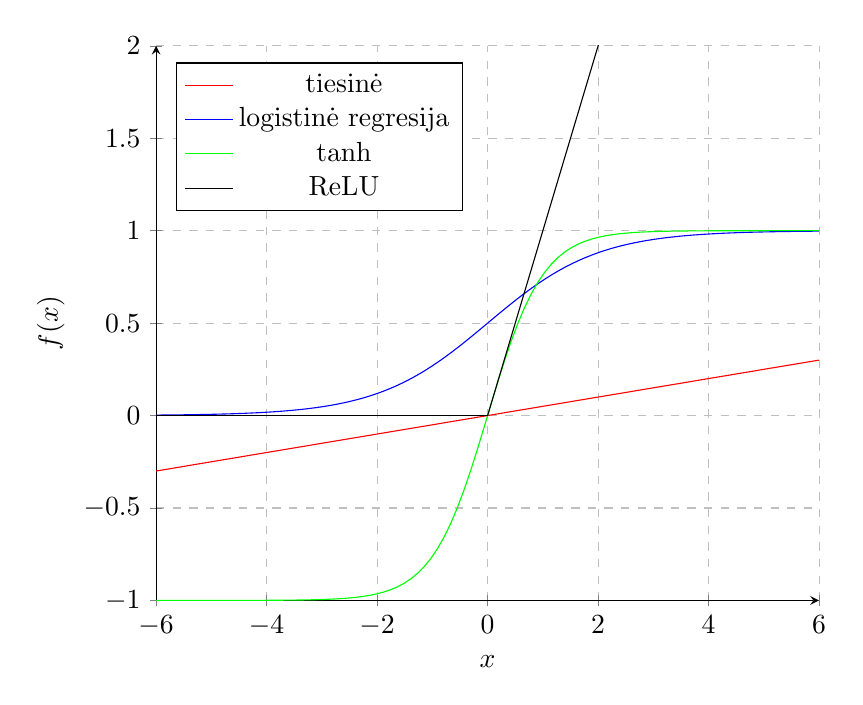
\begin{tikzpicture}
	\begin{axis}[
	axis lines = left,
	width=10cm,
	xlabel = $x$,
	ylabel = {$f(x)$},
	ymax = 2,
	ymajorgrids=true,
	xmajorgrids=true,
	legend pos=north west,
	grid style=dashed,
	]
	%Below the red parabola is defined
	\addplot [
	domain=-6:6, 
	samples=100, 
	color=red,
	]
	{0.05*x};
	\addlegendentry{tiesinė}
	%Here the blue parabloa is defined
	\addplot [
	domain=-6:6,
	samples=100, 
	color=blue,
	]
	{1/(1+exp(-x))};
	\addlegendentry{logistinė regresija}
	
	\addplot [
	domain=-6:6,
	samples=100, 
	color=green,
	]
	{tanh(x)};
	\addlegendentry{tanh}
	
	
	\addplot [
	domain=0:6,
	samples=100, 
	color=black,
	]
	{x};
	\addlegendentry{ReLU}
	
	
	\addplot [
	domain=-6:0,
	samples=100, 
	color=black,
	]
	{0};
	
	\end{axis}
	\end{tikzpicture}
	
	\caption{Aktyvacijos funkcijos} \label{fig:aktyvacijosfunkc}
\end{figure}


\ref{fig:aktyvacijosfunkc} diagramoje pateikiamos šios funkcijos:

\begin{itemize}
	\item Tiesinė – $f(x) = a \cdot x$;
	\item Logistinės regresijos – $f(x) = \frac{1}{1+e^{-x}}$;
	\item Tanh – $f(x) = \tanh(x) = \frac{2}{1+e^{-2x}} - 1$;
	\item ReLU – $f(x) = \begin{cases}
	0 & \text{, kai } x < 0 \\
	x & \text{, kai } x \ge 0
	\end{cases} $.
\end{itemize}

\subsection{Daugiasluosknis perceptronas}

\textbf{Daugiasluoksnis perceptronas} (\textit{angl. multilayer perceptron}) – strukūra, sudaryta iš kelių sluoksnių perceptronų. 

\begin{figure}[H]
	\centering
	\tikzset{%
		every neuron/.style={
			circle,
			draw,
			minimum size=1cm
		},
	}
	
	\begin{tikzpicture}[x=1.5cm, y=1.5cm, >=stealth]
	\centering
	
	\foreach \m/\l [count=\y] in {1,2,3}
	\node [every neuron/.try, neuron \m/.try] (input-\m) at (0,1.9-\y) {};
	
	\foreach \m [count=\y] in {1,2,3,4}
	\node [every neuron/.try, neuron \m/.try ] (hidden-\m) at (2,2.5-\y) {};
	
	\foreach \m [count=\y] in {1,2}
	\node [every neuron/.try, neuron \m/.try ] (output-\m) at (4,2.3-\y*1.6) {};
	
	\foreach \i in {1,...,3}
	\foreach \j in {1,...,4}
	\draw [->] (input-\i) -- (hidden-\j);
	
	\foreach \i in {1,...,4}
	\foreach \j in {1,...,2}
	\draw [->] (hidden-\i) -- (output-\j);
	
	\foreach \l [count=\x from 0] in {Įeigos, Paslėptasis, Išeigos}
	\node [align=center, above] at (\x*2,2) {\l \\ sluoksnis};
	\end{tikzpicture}
	\caption{Daugiasluoksnio perceptrono pavyzdys} \label{fig:ann}
\end{figure}


Dažniausiai daugiasluoksnis perceptronas turi tris ar daugiau sluoksnių – įeigos (\textit{input layer}), paslėptasis (\textit{hidden layer}) ir išeigos (\textit{output layer}) sluoksnių. Paslėptajame sluoksnyje gali būti daugiau nei vienas sluoksnis. Daugiasluoksnis perceptronas kaip aktyvacijos funkciją naudoja nelinijines aktyvacijos funkcijas. Dažniausiai tai būna \textit{tanh} ar loginės regresijos funkcijos. Kiekvienas sluoksnio elementas yra sujungtas su kito sluoksnio elementu, todėl tai sudaro pilnai apjungtą (\textit{angl. fully connected}) tinklą. Yra pavyzdžių, kur daugiausluoksniai perceptronai naudojami atpažinti žodinę kalbą ar versti tekstus.

\subsection{Dirbtiniai neuroniniai tinklai}
\textbf{Dirbtiniai neuroniniai tinklai} (\textit{angl. artificial neural networks}) – struktūra, sukurta remiantis žmogaus nervinės sistemos darbu. Dirbtiniai neuroniniai tinklai gali būti išmokinti atlikti klasifikavimo, spėjimo, sprendimų priėmimo ir kitas užduotis.


Dirbtiniai neuroniniai tinklai remiasi daugiasluoksnio perceptrono principu ir susideda iš šių sluoksnių - įeigos, paslėptojo, kuris gali būti sudarytas iš kelių sluoksnių, ir išeigos.






\subsection{Konvoliuciniai neuroniniai tinklai}

\textbf{Konvoliuciniai neuroniniai tinklai} (\textit{angl. convoliutional neural networks}) – specialios rūšies vienpusiai (\textit{angl. feed-forward}) neuroniniai tinklai, kurie remiasi daugiasluoksnio perceptrono principu. Šie tinklai, kurie remiasi \textit{ReLU} principu yra kelis kartus greitesni, nei tie, kurie remiasi kitais principais, pavyzdžiui, \textit{tanh} \cite{NIPS2012_4824}. Toliau aptariami keli pagrindiniai konvoliucinių neuroninių tinklų sluoksniai.

\subsubsection{Konvoliucinis sluoksnis}

\textbf{Konvoliucinis sluoksnis} (\textit{angl. convoliution layer}) – sluoksnis, skirtas išskirti savybes. Šio sluoksnio 
pritaikymą galima skaidyti į tokias operacijas:


\begin{enumerate}
	\item \textbf{Įeiga}, susidedanti iš $ W_1 \times H_1 \times D_1 $, kur $ W_1 $ - plotis, $ H_1 $ - aukštis ir $ D_1 $ - gylis;
	\item \textbf{Parametrai}, kurie susideda iš $ F $, $ K $, $ P $ ir $ S $, kur:
	\begin{itemize}
		\item $ F $ - filtro dydis (dažniausiai taikomas $ 3 \times 3 $ filtras);
		\item $ K $ - filtrų skaičius (dažniausiai naudojamas  $ 2^n $, kur $ n $ - natūralusis skaičius);
		\item $ P $ - papildomas rėmelis matricai, sudarytas iš 0. Dažniausiai naudojama $ M = \frac{F - 1}{2} $, kur $ M $ yra iš kiekvienos matricos pusės pridedamų eilučių ar stulpelių skaičius, sudarytas iš $0$, tam, kad matrica nepakeistų savo dydžio po šio sluoksnio pritaikymo; 
		\item $ S $ - žingsnis, per kiek paslenkamas filtras (dažniausiai naudojamas $ 1 $);
	\end{itemize}
	\item \textbf{Išeiga}, susidedanti iš $ W_2 \times H_2 \times D_2 $, kur $ W_2 = \frac{W_1 - F + 2P}{S} + 1 $ - plotis, $ H_2 = \frac{H_1 - F + 2P}{S} + 1 $ - aukštis ir $ D_2 = K $ - gylis
\end{enumerate}

\begin{table}[H]\footnotesize
	\centering
	\caption{Pavyzdinės konvoliucinio sluoksnio užduoties ypatybės}
	{\begin{tabular}{| c | c | c | c | c | c | c | c | c | c |} 
		\hline
		\multicolumn{3}{| c |}{\thead{Įeiga}} &
		\multicolumn{4}{ c |}{\thead{Parametrai}} & \multicolumn{3}{ c |}{\thead{Išeiga}} \\
		\hline
		$W_1$ & $H_1$ & $D_1$ & $F$ & $K$ & $P$ & $S$ & $W_2$ & $H_2$ & $D_2$  \\
		\hline
		3 & 3 & 1 & 3 $\times$ 3 & 1 & 1 & 1 & 3 & 3 & 1 \\
		\hline
	\end{tabular}}
	\label{tab:convT}
\end{table}
	
Toliau, \ref{eq:convl} formulėje pateikiamas pavyzdys, kuriame naudojamos \ref{tab:convT} lentelėje pateiktos pavyzdinės konvoliucinio sluoksnio užduoties ypatybės. Spalvos šioje formulėje žymi skirtingų matricų elementus, kur geltona - įeigos matricos elementų spalva, raudona - papildomo rėmelio $P$ spalva, mėlyna - filtro matricos spalva, o žalia - išeigos matricos elemento spalva. \ref{eq:convl1} ir \ref{eq:convl2} formulėse pateikiami konkretūs pavyzdžiai, kuriais remiantis buvo gautos \ref{eq:convl} formulės reikšmės.

\begin{equation}\label{eq:convl}
\begin{bmatrix}
\textcolor{myyellow}{1} & \textcolor{myyellow}{8} & \textcolor{myyellow}{6} \\
\textcolor{myyellow}{9} & \textcolor{myyellow}{2} & \textcolor{myyellow}{4} \\
\textcolor{myyellow}{3} & \textcolor{myyellow}{7} & \textcolor{myyellow}{5}
\end{bmatrix}
\cdot
\begin{bmatrix}
\textcolor{myblue}{1} & \textcolor{myblue}{0} & \textcolor{myblue}{1} \\
\textcolor{myblue}{0} & \textcolor{myblue}{1} & \textcolor{myblue}{0} \\
\textcolor{myblue}{1} & \textcolor{myblue}{0} & \textcolor{myblue}{1}
\end{bmatrix}
=
\begin{bmatrix}
\textcolor{mygreen}{3} & \textcolor{mygreen}{21} & 8 \\
24 & 17 & 19 \\
5 & 20 & 7
\end{bmatrix}
\end{equation}

\begin{equation}\label{eq:convl1}
\textcolor{myred}{0} \cdot \textcolor{myblue}{1}+\textcolor{myred}{0} \cdot \textcolor{myblue}{0}+\textcolor{myred}{0} \cdot \textcolor{myblue}{0}+\textcolor{myred}{0} \cdot \textcolor{myblue}{0}+\textcolor{myyellow}{1} \cdot \textcolor{myblue}{1}+\textcolor{myyellow}{8} \cdot \textcolor{myblue}{0}+\textcolor{myred}{0} \cdot \textcolor{myblue}{1}+\textcolor{myyellow}{9} \cdot \textcolor{myblue}{0}+\textcolor{myyellow}{2} \cdot \textcolor{myblue}{1}=\textcolor{mygreen}{3}
\end{equation}


\begin{equation}\label{eq:convl2}
\textcolor{myred}{0} \cdot \textcolor{myblue}{1}+\textcolor{myred}{0} \cdot \textcolor{myblue}{0}+\textcolor{myred}{0} \cdot \textcolor{myblue}{1}+\textcolor{myyellow}{1} \cdot \textcolor{myblue}{0}+\textcolor{myyellow}{8} \cdot \textcolor{myblue}{1}+\textcolor{myyellow}{6} \cdot \textcolor{myblue}{0}+\textcolor{myyellow}{9} \cdot \textcolor{myblue}{1}+\textcolor{myyellow}{2} \cdot \textcolor{myblue}{0}+\textcolor{myyellow}{4} \cdot \textcolor{myblue}{1}=\textcolor{mygreen}{21}
\end{equation}

\subsubsection{Telkimo sluoksnis}

\textbf{Telkimo sluoksnis} (\textit{angl. pooling layer}) – sluoksnis, skirtas sumažinti matricą, paliekant tik svarbiausias jos dalis. Dažniausiai naudojamos vidutinės (\textit{angl. average pooling}) arba didžiausios (\textit{angl. max pooling}) reikšmės operacijos. 

Telkimo sluoksnio operacijas galima skaidyti į tokias dalis:

\begin{enumerate}
	\item \textbf{Įeiga}, susidedanti iš $ W_1 \times H_1 \times D_1 $, kur $ W_1 $ - plotis, $ H_1 $ - aukštis ir $ D_1 $ - gylis
	\item \textbf{Parametrai}, kurie susideda iš $ F $ ir $ S $, kur $ F $ - filtro dydis (dažniausiai taikomas $ 2 \times 2 $ filtras) ir $ S $ - žingsnis, per kiek paslenkamas filtras (dažniausiai naudojamas $ 2 $)
	\item \textbf{Išeiga}, susidedanti iš $ W_2 \times H_2 \times D_2 $, kur $ W_2 = \frac{W_1 - F}{S} + 1 $ - plotis, $ H_2 = \frac{H_1 - F}{S} + 1 $ - aukštis ir $ D_2 = D_1 $ - gylis
\end{enumerate}


\begin{table}[H]\footnotesize
	\centering
	\caption{Pavyzdinės telkimo sluoksnio užduoties ypatybės}
	{\begin{tabular}{| c | c | c | c | c | c | c | c |} 
		\hline
		\multicolumn{3}{| c |}{\thead{Įeiga}} &
		\multicolumn{2}{ c |}{\thead{Parametrai}} & \multicolumn{3}{ c |}{\thead{Išeiga}} \\
		\hline
		$W_1$ & $H_1$ & $D_1$ & $F$ & $S$ & $W_2$ & $H_2$ & $D_2$  \\
		\hline
		4 & 4 & 1 & 2 $\times$ 2 & 2 & 3 & 3 & 1 \\
		\hline
	\end{tabular}}
	\label{tab:pollT}
\end{table}	
Toliau, \ref{eq:poll} formulėje pateikiamas pavyzdys, kuriame naudojamos \ref{tab:pollT} lentelėje pateiktos pavyzdinės telkimo sluoksnio užduoties ypatybės. Spalvos šioje formulėje žymi filtro su žingsniu pritaikytas operacijas gauti išeigai. \ref{eq:poll1} ir \ref{eq:poll2} formulėse pateikiami konkretūs pavyzdžiai, kuriais remiantis buvo gautos \ref{eq:poll} formulės reikšmės.

\begin{equation}\label{eq:poll}\def\y{\color{myyellow}}\def\b{\color{myblue}}\def\r{\color{myred}}\def\g{\color{mygreen}}
\begin{bmatrix}
\y{1} & \y{3} & \b{1} & \b{3} \\
\y{2} & \y{5} & \b{4} & \b{2} \\
\g{4} & \g{3} & \r{2} & \r{5} \\
\g{2} & \g{5} & \r{4} & \r{2} \\
\end{bmatrix}
= 
\begin{bmatrix}
\y{5} & \b{4} \\
\g{5} & \r{5} 
\end{bmatrix}
\end{equation}
\begin{equation}\label{eq:poll1}
max(
\begin{bmatrix}
\textcolor{myyellow}{1} & \textcolor{myyellow}{3} \\
\textcolor{myyellow}{2} & \textcolor{myyellow}{5}
\end{bmatrix}
) = \textcolor{myyellow}{5}
%1, 3, 1, 3, 2, 5, 2, 4, 3
\end{equation}
\begin{equation}\label{eq:poll2}
max(
\begin{bmatrix}
\textcolor{myblue}{1} & \textcolor{myblue}{3} \\
\textcolor{myblue}{4} & \textcolor{myblue}{2} 
\end{bmatrix}
) = \textcolor{myblue}{4}
\end{equation}

\subsubsection{Atsisakymo sluoksnis}
\textbf{Atsisakymo sluoksnis} (\textit{angl. dropout layer}) – konvoliucinių tinklų sluoksnis, skirtas normalizuoti ir sureguliuoti tarpusavyje susijusių neuronų sąryšius, skirtus perduoti signalus. Mokymo fazėje dažniausiai ištrinamos neuronuose esančios reikšmės tam, kad šis per naują apsimokytų. Galimai netgi atsisakoma tam tikrų neuronų darbo \cite{DBLP:journals/corr/abs-1207-0580}.

\begin{figure}[H]
	\centering
	
	\begin{minipage}{.4\textwidth}
		\centering
		\tikzset{%
			every neuron/.style={
				circle,
				draw,
				minimum size=0.5cm
			},
		}
		
		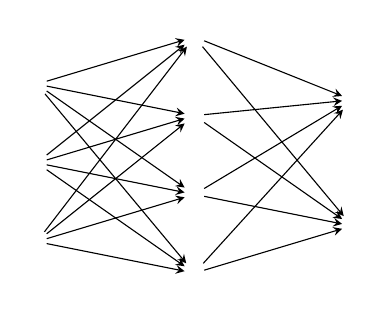
\begin{tikzpicture}[x=1cm, y=1cm, >=stealth]
		\centering
		
		\foreach \m/\l [count=\y] in {1,2,3}
		\node [every neuron/.try, neuron \m/.try] (input-\m) at (0,1.9-\y) {};
		
		\foreach \m [count=\y] in {1,2,3,4}
		\node [every neuron/.try, neuron \m/.try ] (hidden-\m) at (2,2.5-\y) {};
		
		\foreach \m [count=\y] in {1,2}
		\node [every neuron/.try, neuron \m/.try ] (output-\m) at (4,2.3-\y*1.6) {};
		
		\foreach \i in {1,...,3}
		\foreach \j in {1,...,4}
		\draw [->] (input-\i) -- (hidden-\j);
		
		\foreach \i in {1,...,4}
		\foreach \j in {1,...,2}
		\draw [->] (hidden-\i) -- (output-\j);
		
		\end{tikzpicture}
		\caption{Standartinis neuroninis tinklas} \label{fig:snn}
	\end{minipage}
	\begin{minipage}{.4\textwidth}
		\centering
		\tikzset{%
			every neuron/.style={
				circle,
				draw,
				minimum size=0.5cm
			},
			cross/.style={cross out, draw=black, minimum size=2*(#1-\pgflinewidth), inner sep=0pt, outer sep=0pt},
			%default radius will be 1pt. 
			cross/.default={0.19cm},
		}
		
		\begin{tikzpicture}[x=1cm, y=1cm, >=stealth]
		\centering
		
		\foreach \m/\l [count=\y] in {1,2,3}
		\node [every neuron/.try, neuron \m/.try] (input-\m) at (0,1.9-\y) {};
		
		\foreach \m [count=\y] in {1,2,3,4}
		\node [every neuron/.try, neuron \m/.try ] (hidden-\m) at (2,2.5-\y) {};
		
		\foreach \m [count=\y] in {1,2}
		\node [every neuron/.try, neuron \m/.try ] (output-\m) at (4,2.3-\y*1.6) {};
		
		\foreach \i in {1,3}
		\foreach \j in {1,3}
		\draw [->] (input-\i) -- (hidden-\j);
		
		\foreach \i in {1,3}
		\foreach \j in {1,...,2}
		\draw [->] (hidden-\i) -- (output-\j);
		
		\draw (0,-0.1) node[cross] {};
		
		\draw (2,0.5) node[cross] {};
		
		\draw (2,-1.5) node[cross] {};
		\end{tikzpicture}
		\caption{Tinklas po atsisakymo sluoksnio} \label{fig:sdnn}
	\end{minipage}
\end{figure}


\subsection{Rekurentiniai neuroniniai tinklai}

\textbf{Rekurentiniai neuroniniai tinklai} (\textit{angl. recurrent neural networks}) – vienpusiai neuroniniai tinklai, kurie remiasi daugiasluoksnio perceptrono principu. Šie tinklai, apima kitų laiko vienetų apdorotą informaciją ir bendrą kitimą laike \cite{DBLP:journals/corr/Lipton15}.


\begin{figure}[H]
	\centering
	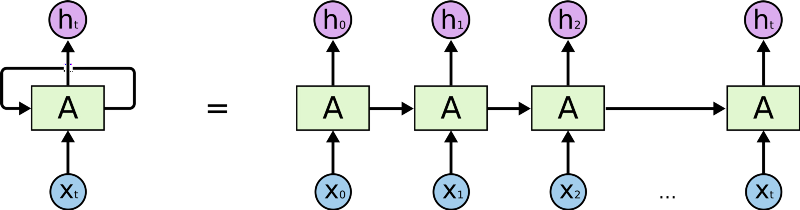
\includegraphics[scale=0.4]{img/rnn}
	\caption{Rekurentinių neuroninių tinklų veikimo principas}
	\label{img:rnn}
\end{figure}

\ref{img:rnn} paveiksėlyje yra pavaizduotas bendrinis rekurentinių neuroninių tinklų veikimo principas, kurį galima užrašyti formule:

\begin{equation}\label{eq:rnn}
h_t = f_w(h_{t-1}, x_t)
\end{equation}

Kur $h_t$ - paslėpto sluoksnio būsena laiko momentu $t$, kurią dar būtų galima vadinti $t$ žingsnio išeiga, $f_w$ - funkcija $f$ su parametrais $w$, $h_{t-1}$ - praėjusio žingsnio būsena, o $x_t$ - įeigos vektorius. Iš šios formulės galima pastebėti, kad kiekviena būsena gauna praeito žingsnio būsena, kuri yra reikalinga norint stebėti būsenas kintant laike	.


\subsubsection{Rekurentinių neuroninių tinklų tipai}

\begin{figure}[H]
	\centering
	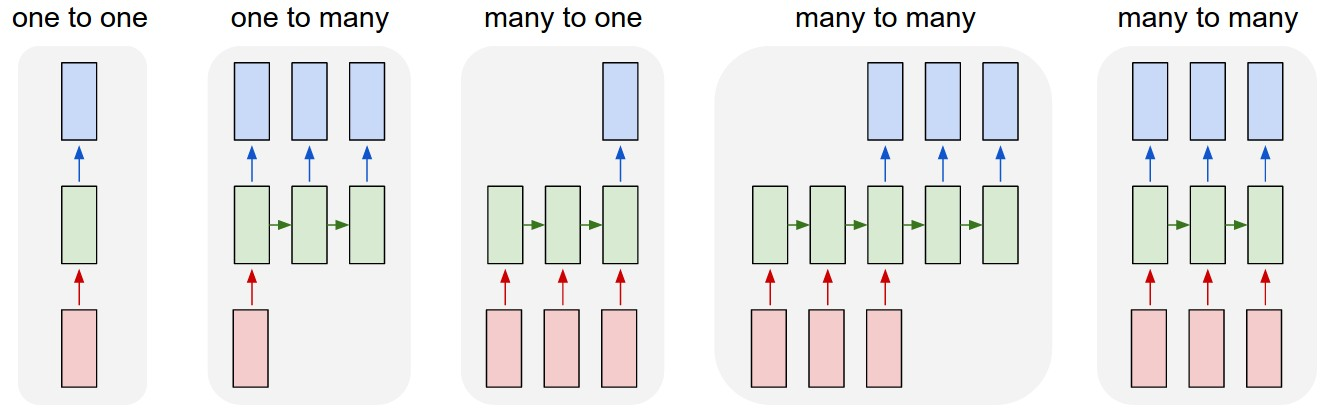
\includegraphics[scale=0.3]{img/nn-tipai}
	\caption{Rekurentinių neuroninių tinklų tipai}
	\label{img:tipai}
\end{figure}

\ref{img:tipai} paveikslėlyje pavaizduoti keturi skirtingi būdai, kuriais naudojantis rekurentiniai neuroniniai tinklai veikia. Rausvos spalvos kvadratėlis reiškia įeigą, žalsvas - paslėptuosius sluoksnius, o melsvas - išeigą. Pateikiami šie būdai:

\begin{itemize}
	\item \textbf{Vienas su vienu} (\textit{angl. one to one}) – būdas, kuriame yra viena įeiga, paslėptasis sluoksnis ir išeiga. Šis būdas dažniausiai taikomas konstruojant konvoliucinius neuroninius tinklus. Kaip pavyzdį galima pateikti paveikslėlio atpažinimą. Tai galėtų būti statinės gestų kalbos atpažinimas;
	\item \textbf{Vienas su daug} (\textit{angl. one to many}) – būdas, kuriame yra viena įeiga, bet kelios išeigos. Vienas iš panaudojimo būdų galėtų būti sakinio suformavimas iš paveikslėlio. Toks tinklas ne tik atpažįsta pagrindinį objektą kadre, bet ir apibūdina esančią aplinką, daro kitus sprendimus;
	\item \textbf{Daug su vienu} (\textit{angl. many to one}) – būdas, kuriame yra daug įeigų, bet tik viena išeiga. Tokio būdo pavyzdys galėtų būti vieno žodžio, tarkime, „labas“ atpažinimas iš video sraudo.
	\item \textbf{Daug su daug} (\textit{angl. many to many}) – būdas, kuriame yra daug įeigų ir daug išeigų. Šis būdas gali būti skaidomas į dvi dalis:
	\begin{itemize}
		\item \textbf{Priklausomas} - įeigų skaičius sutampa su išeigų skaičiumi. Kiekviena įeiga turi savo išeigos atitikmenį. Tai būtų dalinai galima gretitinti su \textit{vienas su vienu} būdu. Pavyzdys šios atšakos galėtų būti video srauto klasifikacija pagal kiekvieną kadrą - nuolatinis atnaujinimas, to kas galėjo būti pasakyta, pavyzdžiui, gestų kalboje.
		\item \textbf{Nepriklausomas} - įeigos skaičius galimai nesutampa su išeigų skaičiumi. Kiekviena įeiga yra nepriklausoma ir išeigos dėliojamos pagal tam tikrus aspektus. Tokio būdo pavyzdys galėtų būti neuroniniai tinklai, kurie atlieka vertėjo funkcijas, pavyzdžiui, iš anglų į lietuvių kalbas, nes skiriasi tiek gramatika, tiek sakinių stilistika.
	\end{itemize}
\end{itemize}

\subsubsection{Rekurentinių neuroninių tinklų modeliai}

Viena pagrindinių problemų, su kuria susiduria paprastieji rekurentiniai neuroniniai tinklai yra nykstančių gradientų problema (\textit{angl. vanishing gradient problem}). Tai problema, kurios metu kiekvieno laiko momentu perceptronas apskaičiuoja naujas reiškmes iš praeitame žingsnyje turimų duomenų ir kaip įeiga priima praeito laiko momento išeigą. 

\begin{equation}
	f(w_n \cdot o_n)=o_{n+1}
\end{equation}

Šioje formulėje $w_n$ - $n$-tojo sluoksnio svoris, $o_n$ - $n$-tojo sluoksnio išeiga, o $f(x)$ - aktyvacijos funkcija.

Tinklo pabaigoje gaunamas praradimas (\textit{angl. loss}) arba kitaip - skirtumas tarp to, kas turėjo būti gauta ir ką tinklas gauna. Sakysime, kad $f(o_n)$ yra praradimas bus funkcija $f$, kurios parametras $o_n$ yra paskutinio sluoksnio išeiga.

Norint pakeisti $w_n$ ($n$-tojo elemento svorį), tai galima padaryti apskaičiuojant gradientą atsižvelgiant į $w_n$.

\begin{equation}
	\frac{\partial Loss}{\partial w_n} = \frac{\partial Loss}{\partial f(o_n)} \cdot \frac{\partial f(o_n)}{\partial w_n} = \frac{\partial Loss}{\partial f(o_n)} \cdot f'(o_n) \cdot w_n
\end{equation}

Čia $frac{\partial Loss}{\partial f(o_n)}$ yra dalinė išvestinė to, kaip skaičiuojamas praradimas. Svarbu tai, kad jis skaičiuojamas iš $f(o_n)$, todėl tai bus pastovi grįžtamojo ryšio (\textit{angl. backpropagation}) lygtis.

Tęsiant toliau pirmojo svorio $w_1$ reikšmę galima apskaičiuoti pagal šią lygtį:

\begin{equation}
\frac{\partial Loss}{\partial w_1} = \frac{\partial Loss}{\partial f(o_n)} \cdot \frac{\partial f(o_n)}{\partial o_{n-1}} \cdots \frac{\partial f(o_2)}{\partial o_1} \cdot \frac{\partial f(o_1)}{\partial w_1} = \frac{\partial f(Loss)}{\partial f(o_n)} \cdot f'(o_n) \cdot w_n \cdots f'(o_1) * w_1
\end{equation}

Dėl šios priežasties ilgainiui dėl per naują skaičiuojamų svorių, perceptronas susiduria su problema, kad „pamiršta“, kas buvo prieš daugiau nei vieną laiko momentą - $w_1$ palaipsniui pradeda nebekisti dėl ilgų skaičiavimų ir tampa labai mažas. Tai reiškia, kad rekurentiniai neuroniniai tinklai paprasčiausiai vadovaujasi trumpalaikės atminties principu. Dėl šios priežasties buvo sukurtos keletas architektūrų, kurios sugebėtų atsiminti ir teisingai įvertinti esamą situaciją. Toliau pateikiami keletos iš tokių neuroninių tinklų architektūrų pavyzdžių.

\subsubsubsection{LSTM}
1997 metais Hochreiter ir Schmidhuber pristatė LSTM modelį, kuris, buvo manyta, galės išspręsti nykstančiųjų gradientų problemą. Šis modelis ypatingas tuo, jog kiekvienas įprastas paslėptojo sluoksnio mazags (\textit{angl. node}) yra pakeistas atminties ląstele \cite{DBLP:journals/corr/Lipton15}.

\textbf{LSTM} – ilga trumpalaikė atmintis (\textit{angl. long short-term memory}) - RNN architektūra, kuri sugeba atsiminti informaciją ilgesniam laiko tarpui. 

Paprasti RNN priima buvusią paslėptąją būseną, pritaiko aktyvacijos funkciją ir grąžina naują būseną. LSTM daro beveik tą patį, tik priima dar ir savo buvusią būseną ir grąžina savo naują būseną. 

LSTM įveda naują sąvoką - vartai (\textit{angl. gate}). LSTM turi trijų skirtingų tipų vartus:

\begin{itemize}
	\item Užmaršties vartai (\textit{angl. forget gate}) - juose apdorojama praeita paslėptoji būsena ir dabartinė įeiga. Šių vartų išeiga - nuosprendis, ką vertėtų pasilikti ląstelės būsenoje, o ką - užmiršti. Kuo vertė artimesnė 1 - tuo tai labiau verta atsiminti, o arčiau 0 - pamiršti.
	\item Įeigos vartai (\textit{angl. input gate}) - įeigos funkcija atnaujina ląstelės būseną.
	\item Išeigos vartai (\textit{angl. output gate}) nusprendžia, kurios ląstelės būsenos reikšmės bus pridedamas į paslėptąją būseną, kuri bus visos ląselės išeiga. Taip pat labai svarbu paminėti ir faktą, kad pasiliekamos ir tos reikšmės ar būsenos, kurios manoma, kad bus reikalingos ateityje.
\end{itemize}


\begin{figure}
	\centering
	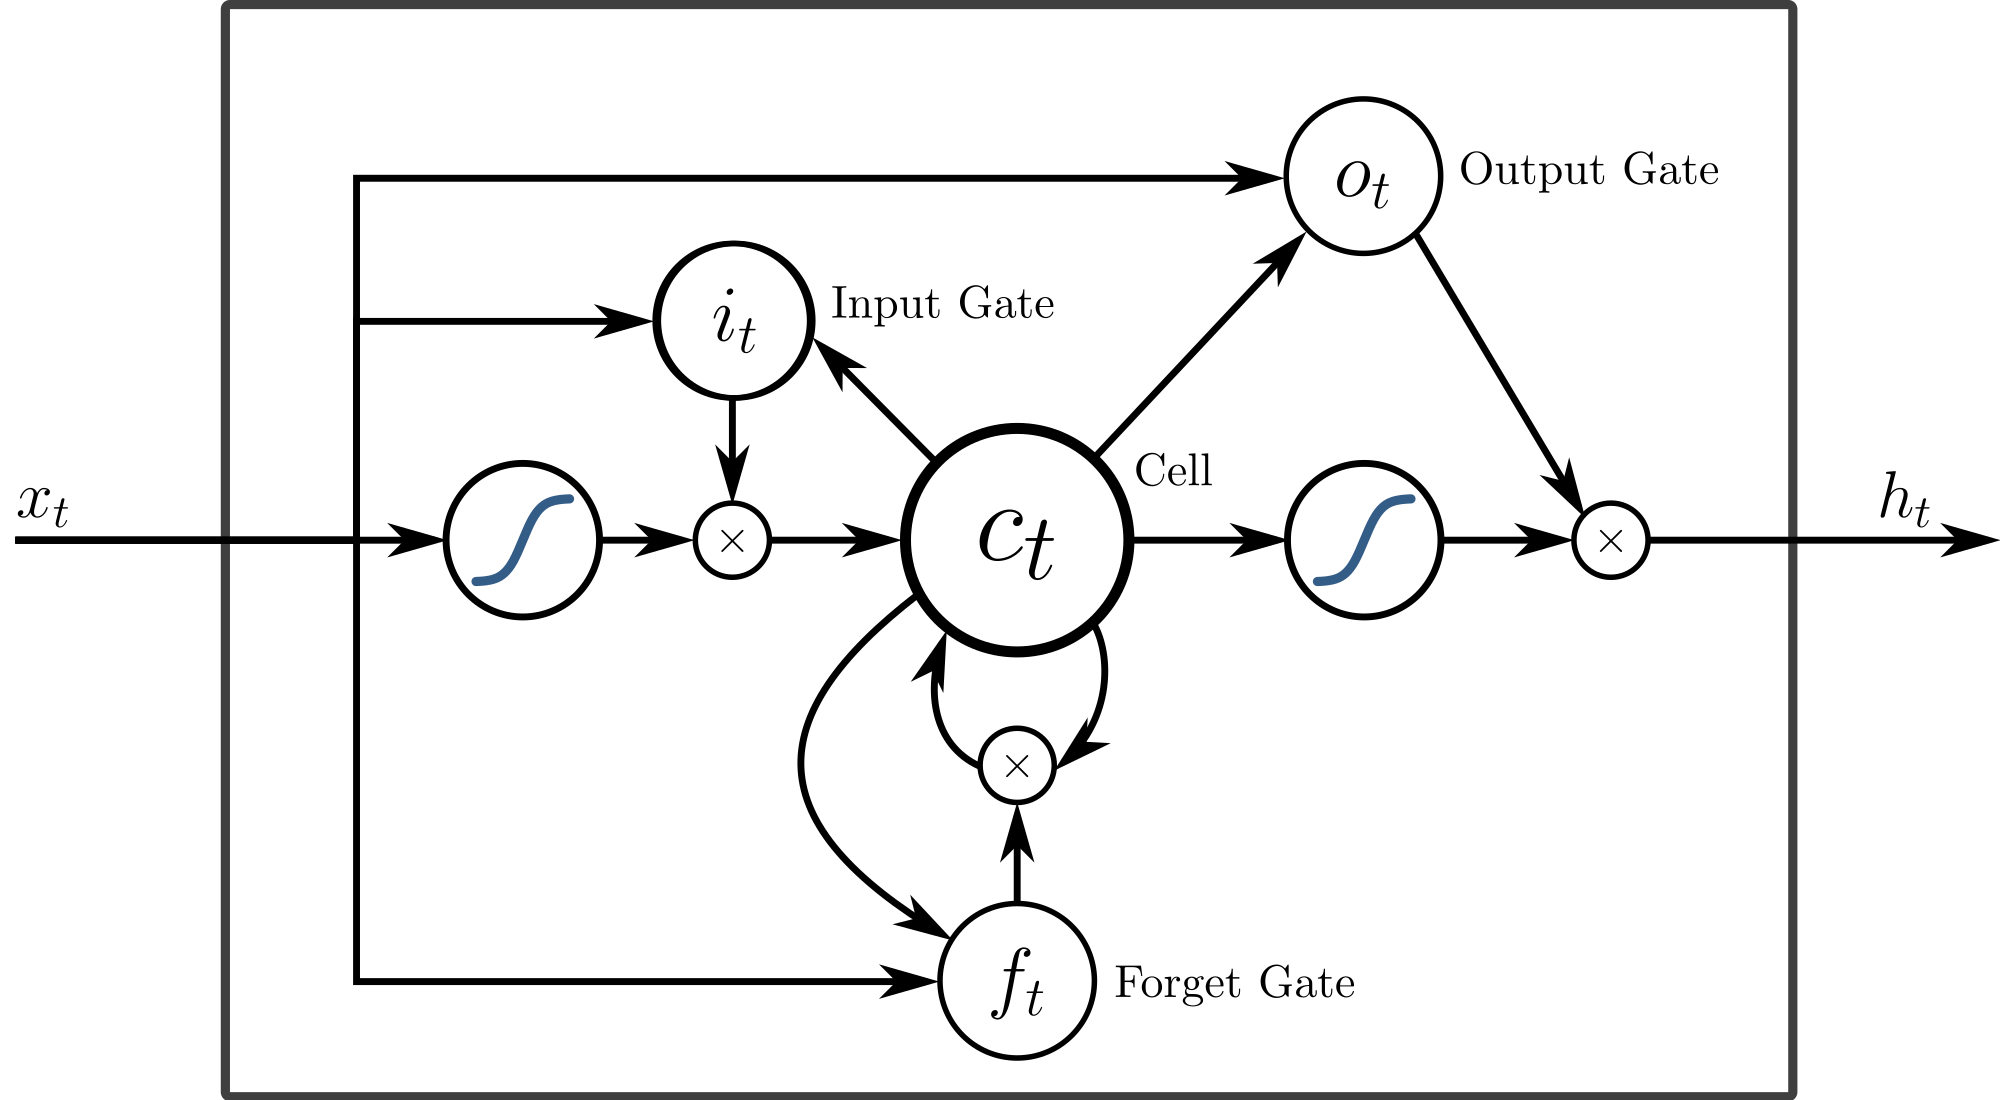
\includegraphics[scale=0.12]{img/lstm}
	\caption{Atminties mazgo pavyzdys}
	\label{img:lstm}
\end{figure}

\subsection{Apjungiamieji tinklų modeliai}

\section{Eksperimentinė dalis}

Šioje dalyje bus aprašomi visi atlikti eksperimentai ir juose gauti rezultatai.

\subsection{Panašūs darbai}
Dar prieš metus, sistemų, kurios atpažintų gestų kalbą konvoliucinių ar rekurentinių tinklų pagalba, beveik nebuvo. 2017 metais Harish Chandra Thuwal ir Adhyan Srivastava iš Jamia Millia Islamia universiteto Naujajame Delyje sukūrė konvoliucinių ir rekurentinių neuroninių tinklų modeliu paremtą sistemą, kuri sugeba atpažinti gestų kalbą iš video srauto. Šiame darbe jie vaizdo įrašą verčia į kadrų seką ir apmoko konvoliucinį tinklą. Vėliau iš šių duomenų apmoko rekurentinį neuroninį tinklą. Svarbu paminėti, kad šie du studentai pasinaudojo argentiniečių gestų kalbos duomenų rinkiniu, kuriame ant kiekvienos rankos žmonės, kurie rodė gestus, buvo užsidėję skirtingų spalvų pirštines. Taip jie iš vaizdo įrašo kadrų ištrindavo visą foną ir palikdavo tik rankas, taip apmokydami sistemą be papildomų savybių.

Naudojantis jų jau sukaupta patirtimi tobulinama sistema galiausiai atpažinti ir lietuvių kalbą.


\subsection{Argentiniečių gestų kalbos atpažinimas}

Buvo pasirinkta apmokyti jau esamą Harish Chandra Thuwal ir Adhyan Srivastava sukurtą modelį, jį tobulinant.

\begin{table}[H]\footnotesize
	\centering
	\caption{Argentiniečių gestų kalbos bandymai su 3 klasėmis}
	{\begin{tabular}{| c | c | c | c | c | c | c |} \hline
		\thead{Bandymo\\Nr.} & \thead{Klasių\\skaičius} & \thead{Apmokymo\\tikslumas} & \thead{Epochų\\skaičius} & \thead{Tikslumas} & \thead{Praradimas} & \thead{Testavimas}  \\
		\hline
		1. & 3 & 100\% & 10 & 81.27\% & 0.6431 & 85.32\% \\
		\hline
		2. & 3 & 99.99\% & 100 & 89.27\% & 0.4422 & 93.33\% \\
		\hline
	\end{tabular}}
	\label{tab:asl-bandymai1}
\end{table}


\begin{table}[H]\footnotesize
	\centering
	\caption{Argentiniečių gestų kalbos bandymai su 25 klasėmis}
	{\begin{tabular}{| c | c | c | c | c | c | c |} \hline
		\thead{Bandymo\\Nr.} & \thead{Klasių\\skaičius} & \thead{Apmokymo\\tikslumas} & \thead{Epochų\\skaičius} & \thead{RNN\\apmokymo\\tipas} & \thead{Tikslumas} & \thead{Praradimas}  \\
		\hline
		1. & 25 & 91.90\% & 100 & Platus & 91.99\% & 0.6839 \\
		\hline
		2. & 25 & 91.90\% & 100 & Platesnis & 91.95\% & 0.6255 \\
		\hline
		3. & 25 & 91.90\% & 100 & Gilus & 16.55\% & 2.0566 \\
		\hline
		4. & 25 & 91.90\% & 10 & Paprastas & 97.61\% & 0.2814 \\
		\hline
		5. & 25 & 91.90\% & 100 & Paprastas & 92.66\% & 0.5539 \\
		\hline
	\end{tabular}}
	\label{tab:asl-bandymai2}
\end{table}


\subsection{Lietuvių gestų kalbos atpažinimas}

Lietuvių kalbai su gestų kalbos atpažinimu naudojantis konvoliuciniais ar rekurentiniais neuroniniais tinklais oficialaus nieko nėra. Todėl toliau pateikiama, kas buvo atlikta ir kokie rezultatai buvo gauti naudojantis šiais metodais jau anksčiau aptartu ir perdarytu modeliu. 

\subsubsection{Duomenų paruošimas}
Lietuvių gestų kalbos žodyne pateikiama apie 9000 gestų. Žodynas rengiamas nuo 2004 metų kurčiųjų ir girdinčiųjų komandos. Šiame žodyne gestus galima rasti pagal žodį, gesto formą ar temą. Taip pat galima pasirinkti ar gesto ieškoti kaip atitinkamo žodžio ar naudojimo pavyzdžiuose. Susiradus tinkamą žodį yra aprašomos tokios specifikos kaip plaštakos forma, lūpų judesys, žodžio ar sakinio reikšmė. Tačiau iškyla viena problema - kiekvienas gestas turi tik po vieną video įrašą atitinkantį tą žodį. Toks kiekis duomenų yra per mažas, norint apmokyti sistemą. Galima iš sakinių, kuriuose yra žodžio naudojimo pavyzdžiai, taip pat išsikirpti gestus, atitinkančius norimą gestą. Tačiau tai padidintų kiekvienos klasės duomenų kiekį iki daugiausiai 5 vaizdo įrašų. Net ir toks duomenų kiekis yra per mažas.

Nuspręsta duomenis susikurti pačiam. Teko pramokti lietuvių gestų kalbos gestus. Įsigilinti į gestų kalbos specifiką. Pirmiesiems bandymams buvo nufilmuota 3 skirtingų žodžių klasių gestai po 50 video įrašų kiekvienam. Filmuota buvo mobiliuoju telefonu atistojus prie gelsvos sienos. Filmuoti buvo du skirtingi asmenys.


\subsubsection{Modelio apmokymas}

\begin{itemize}
	\item 3 klasės 45 kiekvienai klasei. bendrai 145
	\item 121 training samples, 14 validation, 100 epochs, 86.93\% accuracy, 0.5081 total loss
	\item 92.31\% tikslumas iš nematytų 13 video.
\end{itemize}

\subsubsection{Modelio testavimas}


\section{Medžiagos darbo tema dėstymo skyriai}
Medžiagos darbo tema dėstymo skyriuose išsamiai pateikiamos nagrinėjamos temos
detalės: pradiniai duomenys, jų analizės ir apdorojimo metodai, sprendimų
įgyvendinimas, gautų rezultatų apibendrinimas.

Medžiaga turi būti dėstoma aiškiai, pateikiant argumentus. Tekste dėstomas
trečiuoju asmeniu, t.y. rašoma ne „aš manau“, bet „autorius mano“, „autoriaus
nuomone“. Reikėtų vengti informacijos nesuteikiančių frazių, pvz., „...kaip jau
buvo minėta...“, „...kaip visiems žinoma...“ ir pan., vengti grožinės
literatūros ar publicistinio stiliaus, gausių metaforų ar panašių meninės
išraiškos priemonių.

Skyriai gali turėti poskyrius ir smulkesnes sudėtines dalis, kaip punktus ir
papunkčius.
%Citavimo pavyzdžiai: cituojamas vienas šaltinis \cite{PvzStraipsnLt}; cituojami
%keli šaltiniai \cite{PvzStraipsnEn, PvzKonfLt, PvzKonfEn, PvzKnygLt, PvzKnygEn,
%PvzElPubLt, PvzElPubEn, PvzMagistrLt, PvzPhdEn}.


\sectionnonum{Rezultatai ir išvados}
Rezultatų ir išvadų dalyje išdėstomi pagrindiniai darbo rezultatai (kažkas
išanalizuota, kažkas sukurta, kažkas įdiegta), toliau pateikiamos išvados
(daromi nagrinėtų problemų sprendimo metodų palyginimai, siūlomos
rekomendacijos, akcentuojamos naujovės). Rezultatai ir išvados pateikiami
sunumeruotų (gali būti hierarchiniai) sąrašų pavidalu. Darbo rezultatai turi
atitikti darbo tikslą.

\printbibliography[heading=bibintoc]  % Šaltinių sąraše nurodoma panaudota
% literatūra, kitokie šaltiniai. Abėcėlės tvarka išdėstomi darbe panaudotų
% (cituotų, perfrazuotų ar bent paminėtų) mokslo leidinių, kitokių publikacijų
% bibliografiniai aprašai. Šaltinių sąrašas spausdinamas iš naujo puslapio.
% Aprašai pateikiami netransliteruoti. Šaltinių sąraše negali būti tokių
% šaltinių, kurie nebuvo paminėti tekste. Šaltinių sąraše rekomenduojame
% necituoti savo kursinio darbo, nes tai nėra oficialus literatūros šaltinis.
% Jei tokių nuorodų reikia, pateikti jas tekste.

\sectionnonum{Sutartiniai žymėjimai}

\begin{itemize}
	\item $i_t$ – įeiga laiko momentu $t$
	\item $o_t$ – išeiga laiko momentu $t$
	\item $h_t$ – būsena laiko momentu $t$
\end{itemize}


\sectionnonum{Sąvokų apibrėžimai}

\begin{itemize}
	\item Dirbtiniai neuroniniai tinklai - artificial neural networks
	\item Inception v3 - Google modelis
	\item Išeiga - output
	\item Įeiga - input
	\item Konvoliuciniai neuroniniai tinklai - convolutional neural networks
	\item Neuroniniai tinklai - neural networks
	\item Paslėptasis sluoksnis - hidden layer
	\item Rekurentiniai neuroniniai tinklai - recurrent neural networks
	\item Sluoksnis - layer
	\item Vienpusiai neuroniniai tinklai - Feed-Forward neural networks
\end{itemize}

\sectionnonum{Santrumpos}
\begin{itemize}
	\item KNN - konvoliuciniai neuroniniai tinklai
	\item NN - neuroniniai tinklai
	\item RNN - Rekurentiniai neuroniniai tinklai
	
\end{itemize}

Sąvokų apibrėžimai ir santrumpų sąrašas sudaromas tada, kai darbo tekste
vartojami specialūs paaiškinimo reikalaujantys terminai ir rečiau sutinkamos
santrumpos.

\appendix  % Priedai
% Prieduose gali būti pateikiama pagalbinė, ypač darbo autoriaus savarankiškai
% parengta, medžiaga. Savarankiški priedai gali būti pateikiami ir
% kompaktiniame diske. Priedai taip pat numeruojami ir vadinami. Darbo tekstas
% su priedais susiejamas nuorodomis.

\section{Rankų pirštų numeracija}
\label{appendix:pirstai}
\begin{figure}[H]
    \centering
    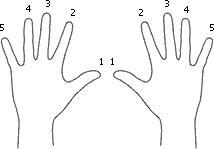
\includegraphics[scale=1]{img/fingers}
    \caption{Kairės ir dešinės rankų pirštų numeracija}
    \label{img:fingers}
\end{figure}

\section{Konvoliucinio tinklo modelis}
\label{appendix:inception_v3}
\begin{figure}[H]
	\centering
	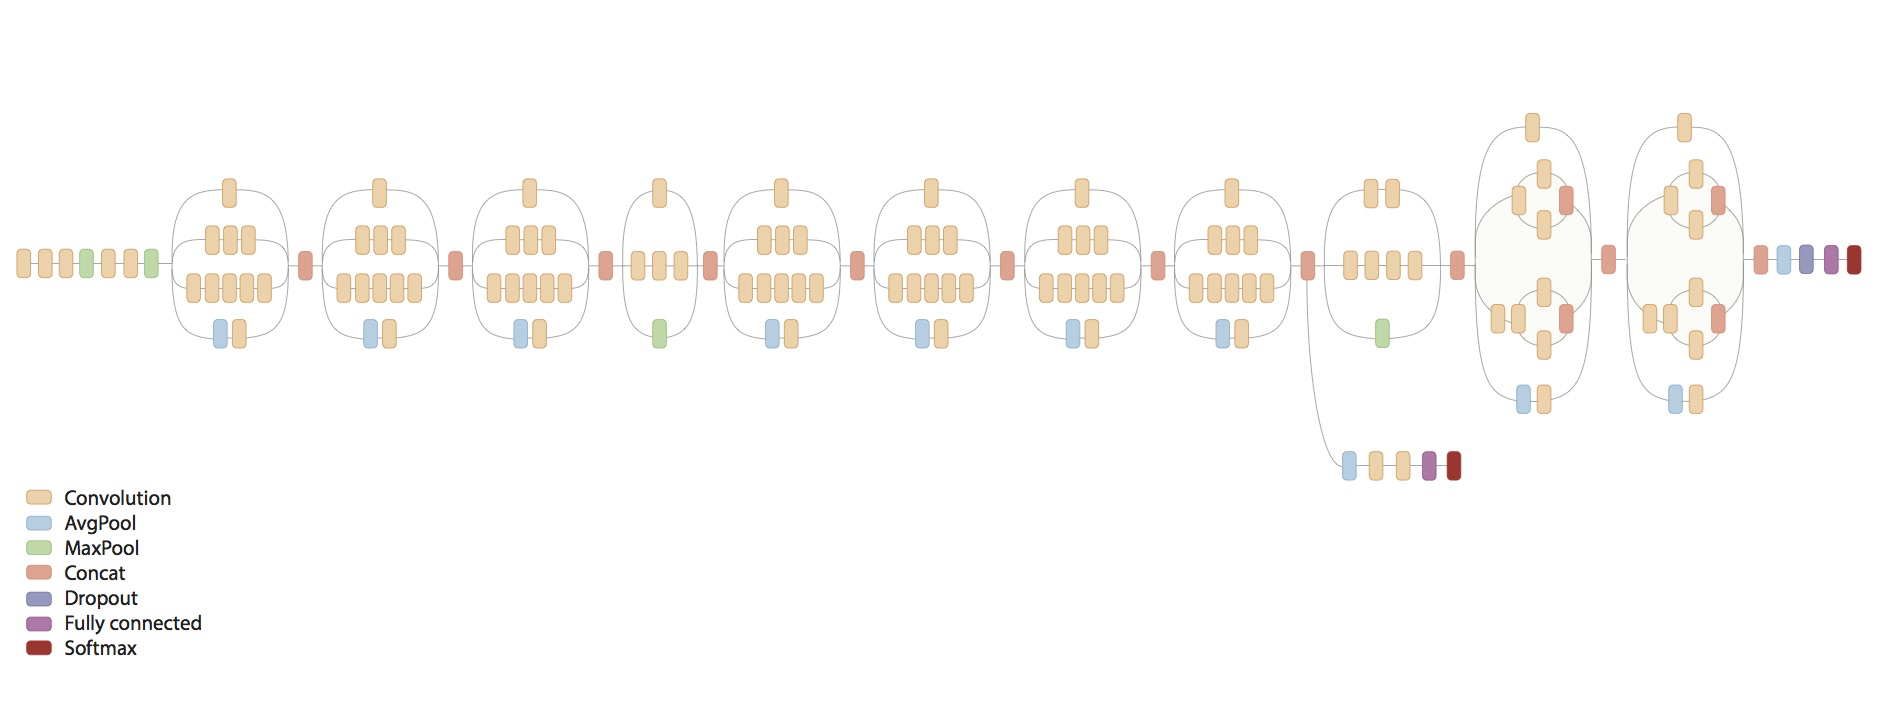
\includegraphics[scale=0.2]{img/inception_v3}
	\caption{Konvoliucinio tinklo modelis „Inception v3“}
	\label{img:inception_v3}
\end{figure}

%\section{Eksperimentinio palyginimo rezultatai}
%% tablesgenerator.com - converts calculators (e.g. excel) tables to LaTeX
%\begin{table}[H]\footnotesize
%  \centering
%  \caption{Lentelės pavyzdys}
%  {\begin{tabular}{|l|c|c|} \hline
%    Algoritmas & $\bar{x}$ & $\sigma^{2}$ \\
%    \hline
%    Algoritmas A  & 1.6335    & 0.5584       \\
%    Algoritmas B  & 1.7395    & 0.5647       \\
%    \hline
%  \end{tabular}}
%  \label{tab:table example}
%\end{table}

\end{document}
